\documentclass{article}

% if you need to pass options to natbib, use, e.g.:
% \PassOptionsToPackage{numbers, compress}{natbib}
% before loading nips_2017
%
% to avoid loading the natbib package, add option nonatbib:
% \usepackage[nonatbib]{nips_2017}

\usepackage{nips_2017}

% to compile a camera-ready version, add the [final] option, e.g.:
% \usepackage[final]{nips_2017}

\usepackage[utf8]{inputenc} % allow utf-8 input
\usepackage[T1]{fontenc}    % use 8-bit T1 fonts
\usepackage{hyperref}       % hyperlinks
\usepackage{url}            % simple URL typesetting
\usepackage{booktabs}       % professional-quality tables
\usepackage{amsfonts}       % blackboard math symbols
\usepackage{nicefrac}       % compact symbols for 1/2, etc.
\usepackage{microtype}      % microtypography
% set imports
\usepackage{ntheorem}       % theorem writing
\usepackage{cleveref}       % clever references
\usepackage{graphicx}       % for images
\usepackage[table,xcdraw]{xcolor} % for tables
\usepackage{natbib}            % bibliography
\usepackage{amsmath, amssymb}  % math
\usepackage{bm}                % ?
\usepackage{subcaption}        % images
\usepackage{hyperref}          % linked refs

% set paths
\graphicspath{{./fig/}}

\title{Attacking Speaker Recognition with \\Deep Generative Models}
% The \author macro works with any number of authors. There are two
% commands used to separate the names and addresses of multiple
% authors: \And and \AND.
%
% Using \And between authors leaves it to LaTeX to determine where to
% break the lines. Using \AND forces a line break at that point. So,
% if LaTeX puts 3 of 4 authors names on the first line, and the last
% on the second line, try using \AND instead of \And before the third
% author name.

\author{
  Anish Doshi \\
  UC Berkeley \\
  Berkeley, 94709 \\
  \texttt{apdoshi@berkeley.edu} \\
  \And
  Wilson Cai\\
  UC Berkeley\\
  Berkeley, 94709 \\
  \texttt{wcai@berkeley.edu} \\
  \And
  Rafael Valle \\
  Center for New Music and Audio Technologies \\
  UC Berkeley\\
  \texttt{rafaelvalle@berkeley.edu} \\
}

\begin{document}
% \nipsfinalcopy is no longer used

\maketitle

\begin{abstract}
    In this paper we investigate the ability of generative adversarial networks (GANs) to synthesize spoofed attacks on modern speaker recognition systems. We first show that the modern architectures of SampleRNN 
    and WaveNet are unable to fool CNN-based speaker recognition systems. We propose  
    a modification of the Wasserstein GAN objective function to make use of data that is 
    real but not from the class being learned. Our method is able to perform both targeted and untargeted attacks against state of the art systems, which calls attention to issues related with security. 
\end{abstract}

% setup theorems 
\theoremseparator{:}
\newtheorem{hyp}{Hypothesis}

\section{Introduction} \label{sec:introduction}
Speaker recognition and authentication systems are being deployed for security
critical applications such as banking, forensics, home automation, etc. Like
other domains, these systems benefit from recent advancements in deep
learning that lead to improved accuracy and trainability of such systems.
Despite the improvement in the efficiency of these systems, evidence shows that
they can be suspectible to adversarial attacks\cite{wu2015spoofing}, thus motivating a current trend
focused understanding adversarial attacks (\cite{szegedy2013intriguing}, \cite{goodfellow2014explaining}) and finding countermeasures to detect of deflect them. 

Parallel to these advancements, neural speech \textit{generation} (the process of using deep neural networks to generate human-sounding speech) has also seen huge progress (\cite{wang2017tacotron}, \cite{arik2017deep}). Generative Adversarial Networks (GANs) have recently been found to produce incredibly  authentic samples in a variety of fields. The core idea of GANs - namely the minimax game played between a generator network and a discriminator network - extends very naturally to the field of speaker authentication and spoofing. \\
The combination of these advancements begs a natural question that has, to the
best of our knowledge, not been answered:
\begin{center}
Are state-of-the-art speech recognition systems robust \\to adversarial attacks by speech generative models?
\end{center}

More specifically, we contemplate this question and offer in this paper the following contributions:
\begin{itemize}
\item We evaluate SampleRNN and WaveNet in their ability to fool text-independent state-of-the-art speaker recognizers.
\item We propose strategies for untargeted attacks using Generative Adversarial Networks.
\item We propose strategies for targeted attacks using a new objective function based on the improved Wasserstein GAN.
\end{itemize}

%
\section{Related work}\label{sec:related_work}
Modern generative models are sophisticated enough to produce fake\footnote{We use the term fake to refer to
computer generated samples} speech samples that can be indistinguishable from real human speech. Here, we provide a summary of some existing neural speech synthesis models and their architectures.
WaveNet~\cite{van2016wavenet} is a generative neural network that is trained end-to-end
to model quantized audio waveforms. The model is fully
probabilistic and autoregressive, using a stack of causal convolutional layers
to condition the predictive distribution for each audio sample on all previous ones. It has produced impressive results for generation of speech audio conditioned on speaker and text and has become a standard baseline for neural speech generative models. 

SampleRNN~\cite{mehri2016samplernn} is another autoregressive architecture that
has been successfully used to generate both speech and music samples. SampleRNN
uses a hierarchical structure of deep RNNs to model dependencies in the sample
sequence. Each deep RNN operates at a different temporal resolution so as to
model both long term and short term dependencies. 


Recent work on deep learning architectures has also introduced the presence of \textit{adversarial examples}: small perturbations to the original inputs, normally imperceptible to humans, which nevertheless cause the architecture to generate an incorrect or deliberately chosen output. In their brilliant papers, ~\cite{szegedy2013intriguing} and
~\cite{goodfellow2014explaining} analyze the origin of adversarial attacks and
describe simple and very efficient techniques for creating such perturbations, such as the fast gradient sign method. 

In the vision domain, ~\cite{sharif2016accessorize} describe a technique for attacking facial recognition systems. Their attacks are physically realizable and inconspicuous, allowing an attacker to impersonate another individual. In the speech domain,~\cite{carlini2016hidden} describe attacks on speech-recognition systems which use sounds that are hard to recognize by humans but interpreted as specific commands by speech-recognition systems.

To the best of our knowledge, GANs have not been used before for the purpose of speech synthesis. \cite{pascual2017segan} uses a conditional GAN for the purpose of speech \textit{enhancement}, i.e. taking as input a raw speech signal and outputting a denoised waveform. The model in \cite{chang2017learning} tackles the reverse problem of using GANs to learn certain representations given a speech spectrogram. We believe the use of spectrograms is a step in the right direction of GAN speech research, as using the raw waveform as input has highlighted current issues with using GANs with sequential modeling.
%
\section{Data}\label{sec:method}
In this section we will describe the datasets used and the pipeline, including pre-processing and feature extraction, 

\subsection{Datasets}
In our experiments we use three datasets, each assigned to a model as described in Table\ref{tbl:datasets}. The datasets used are public and provide audio clips of different lengths and quality.

\begin{table}[!h]
\centering
\caption{Description of datasets used in our experiments. Book narr. refers to book narratives. Newspaper ++ refers to newspapers and other documents. Conversational tel. refers to conversational telephone speech.}
\label{tbl:datasets}
\begin{tabular}{llllll}
                                                                     & \cellcolor[HTML]{C0C0C0}Speakers & \cellcolor[HTML]{C0C0C0}Language & \cellcolor[HTML]{C0C0C0}Duration & \cellcolor[HTML]{C0C0C0}Context & \cellcolor[HTML]{C0C0C0}Model \\ \cline{2-6} 
\multicolumn{1}{l|}{\cellcolor[HTML]{C0C0C0}2013 Blizzard} & 1                                & English                          & 73 h                             & Book narr.                  & SampleRNN                     \\
\multicolumn{1}{l|}{\cellcolor[HTML]{C0C0C0}CSTR VCTK}               & 109                              & English                          & 400 Sentences                    & Newspaper ++               & WaveNet                       \\
\multicolumn{1}{l|}{\cellcolor[HTML]{C0C0C0}2004 NIST}               & 100                              & Multiple                         & 5 min / speaker                  & Conversational tel. & WGAN                         
\end{tabular}
\end{table}

\subsection{Pre-processing}
\label{sub:processdata}
Data pre-processing is dependent on the model being trained. For SampleRNN and WaveNet, the raw audio is reduced to 16kHz and quantized using the $\mu-law$ companding transformation as referenced in SampleRNN~\cite{mehri2016samplernn} and WaveNet~\cite{van2016wavenet}. For the model based on the Wasserstein GAN, we pre-process the data by converting it to 16kHz and removing silences by using the WebRTC Voice Activity Detector (VAD) as referenced in~\cite{zeidan2014webrtc}.

\subsection{Feature extraction}
SampleRNN and WaveNet operate at the sample level, i.e. waveform, thus requiring no feature extraction.
The features used for the neural speaker recognition system is based on Mel-Spectrograms with dynamic range compression. The Mel-Spectrogram is obtained by projecting a spectrogram onto a mel scale. We use the python library librosa~\cite{mcfee2015librosa} to project the spectrogram onto 64 mel bands, with window size equal to 1024 samples and hop size equal to 160 samples, i.e. frames of 100ms long. Dynamic range compression is computed as described in~\cite{lukic2016speaker}, with $log(1 + C*M)$, where $C$ is the a compression constant scalar set to $1000$ and $M$ is the matrix representing the Mel-Spectrogram.
                        
\section{Classification Model}
\subsection{Gaussian Mixture Model - Universal Background Model}
\subsection{Neural speaker recognition system}
The speaker recognition system used in our experiments is based on the state-of-the-art framework by \cite{lukic2016speaker} and is described in Figure \ref{fig:CNN}. The first module at the bottom is a pre-processing step that extracts Mel-Spectrograms features from the waveform as described in section \ref{sub:processdata}. The second module is a convolutional neural network (CNN) that performs multi-speaker classification using the Mel-Spectrograms. The CNN is a modified version of Alexnet~\cite{krizhevsky2012imagenet}.

\begin{figure}[h]
    \centering
    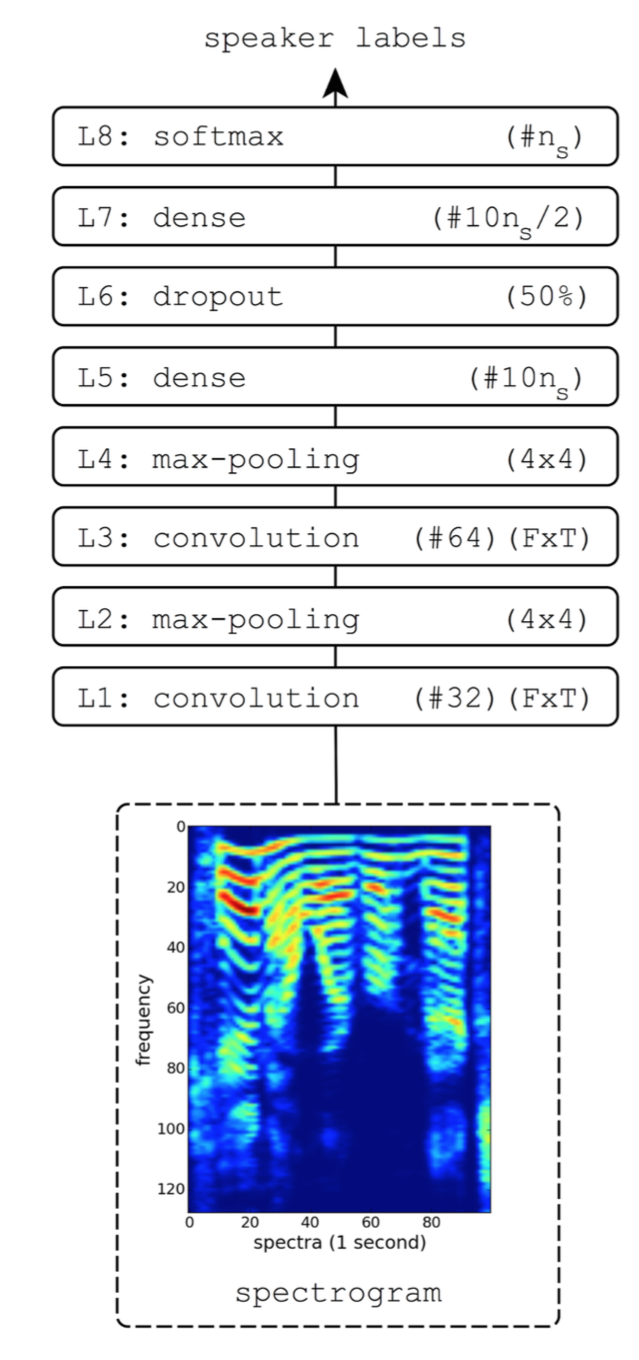
\includegraphics[width=0.25\textwidth]{./fig/cnn.png}
    \caption{Architecture for CNN speaker verifier}
    \label{fig:CNN}
\end{figure}

We train the CNN on our training set using 64*64 Mel-Spectrograms~\footnote{64 mel bands and 64 frames, 100 ms each} consisting of balanced samples from 101 speakers from the NIST 2004 and Blizzard datasets. Our model achieves 85\% test set accuracy.

\section{Generative Model}
\subsection{WaveNet} % (fold)
\label{sub:WaveNet}
WaveNet is a generative neural network trained end-to-end to model quantized audio waveforms. It has produced impressive results for conditional, speaker and text, generation of speech audio. The model is fully probabilistic and autoregressive, using a stack of causal convolutional layers to condition the predictive distribution for each audio sample on all previous ones;
\subsection{SampleRNN}
SampleRNN \cite{mehri2016samplernn}, another autoregressive architecture that has been successfully used to generate both speech and music samples. SampleRNN uses a hierarchical structure of deep RNNs to model dependencies in the sample sequence. Each deep RNN operates at a different temporal resolution so as to model both long term and short term dependencies.  
\subsection{Wasserstein GANs} % (fold)
\label{sub:Wasserstein_GANsh}
In the original generative adversarial network (GAN) framework proposed by \cite{goodfellow2014generative}, a \textit{generator} network is trained to learn a function from noise to samples that approximate the real data distribution. Simultaneously, a \textit{discriminator} network is trained to identify whether a sample came from the real distribution or not - i.e., it is trained to try to output 1 if a sample is real, and 0 if a sample is fake. The generator and discriminator can be arbitrary networks. \\
The GAN framework has been shown to be able to produce very realistic samples with low training overhead. However, since the generator is trained to minimize the Kullback-Leibler (KL) divergence between its constructed distribution and the real one, it suffers from an exploding loss term when the real distribution's support isn't contained in the constructed one. To counter this, the \textit{Wasserstein GAN} \cite{arjovsky2017wasserstein} (WGAN) framework instead uses the Wasserstein (Earth-Mover) distance between distributions instead, which in many cases does not suffer from the same explosion of loss and gradient. Based on this, the loss functions of the generator and \textit{critic} (which no longer emits a simple probability, but rather an approximation of the Wasserstein distance between the fake distribution and real) become:
\begin{align}
    L_G &= -\underset{\boldsymbol{\widetilde{x}} \sim \mathbb{P}_{g}}{\mathbb{E}}  \big[D(\boldsymbol{\widetilde{x}})\big] \\
    L_C &= \underset{\boldsymbol{\widetilde{x}} \sim \mathbb{P}_{g}}{\mathbb{E}}  \big[D(\boldsymbol{\widetilde{x}})\big] - \underset{\boldsymbol{x} \sim \mathbb{P}_{r}}{\mathbb{E}}  \big[D(\boldsymbol{x})\big]
\end{align}
where $P_r$ is the real distribution, and $P_g$ the learnt distribution of the generator. \\
The original WGAN framework uses weight clipping to ensure that the critic satisfies a Lipschitz condition. As pointed by \cite{gulrajani2017improved}, however, this clipping can lead to problems with gradient stability. Instead, \cite{gulrajani2017improved} suggest adding a gradient penalty to the critic's loss function, which indirectly tries to constrain the original critic's gradient to have norm close to 1. Equation (2) thus becomes (taken from \cite{gulrajani2017improved}):
\begin{align}
    L_C &= \underbrace{\underset{\boldsymbol{\widetilde{x}} \sim \mathbb{P}_{g}}{\mathbb{E}}  \big[D(\boldsymbol{\widetilde{x}})\big] - \underset{\boldsymbol{x} \sim \mathbb{P}_{r}}{\mathbb{E}}  \big[D(\boldsymbol{x})\big]}_\text{Original critic loss}  + \underbrace{\lambda \underset{\boldsymbol{\hat{x}} \sim \mathbb{P}_{\hat{x}}}{\mathbb{E}}  \big[(\lVert \nabla_{\boldsymbol{\hat{x}}} D(\boldsymbol{\hat{x}}) \rVert_2 - 1)^2\big]}_\text{Gradient Penalty}
\end{align}

% subsection wgan_approach (end)
\subsection{Adversarial attacks}
Attacks to classification systems can be targeted or untargeted. In targeted attacks, an adversary is interested in producing an adversarial input that makes the classification system predict a target class. In untargeted attacks, the adversary is interest in a confident prediction, regardless of the class.

%
\section{Attacking speaker recognition models}\label{sec:spk_rec_atks}
In this section, we define adversarial attacks on speaker recognition models, and describe the methodology we use to perform them.

\subsection{Neural speaker recognition system}
\label{sub:speaker_recognition}
The speaker recognition system used in our experiments is based on the state-of-the-art framework by \cite{lukic2016speaker} and is described in Figure \ref{fig:CNN}. The first module at the bottom is a pre-processing step that extracts the Mel-Spectrogram from the waveform as described in section \ref{sub:processdata}. The second module is a convolutional neural network (CNN) that performs multi-speaker classification using the Mel-Spectrogram. The CNN is a modified version of Alexnet~\cite{krizhevsky2012imagenet}.

\begin{figure}[h]
    \centering
    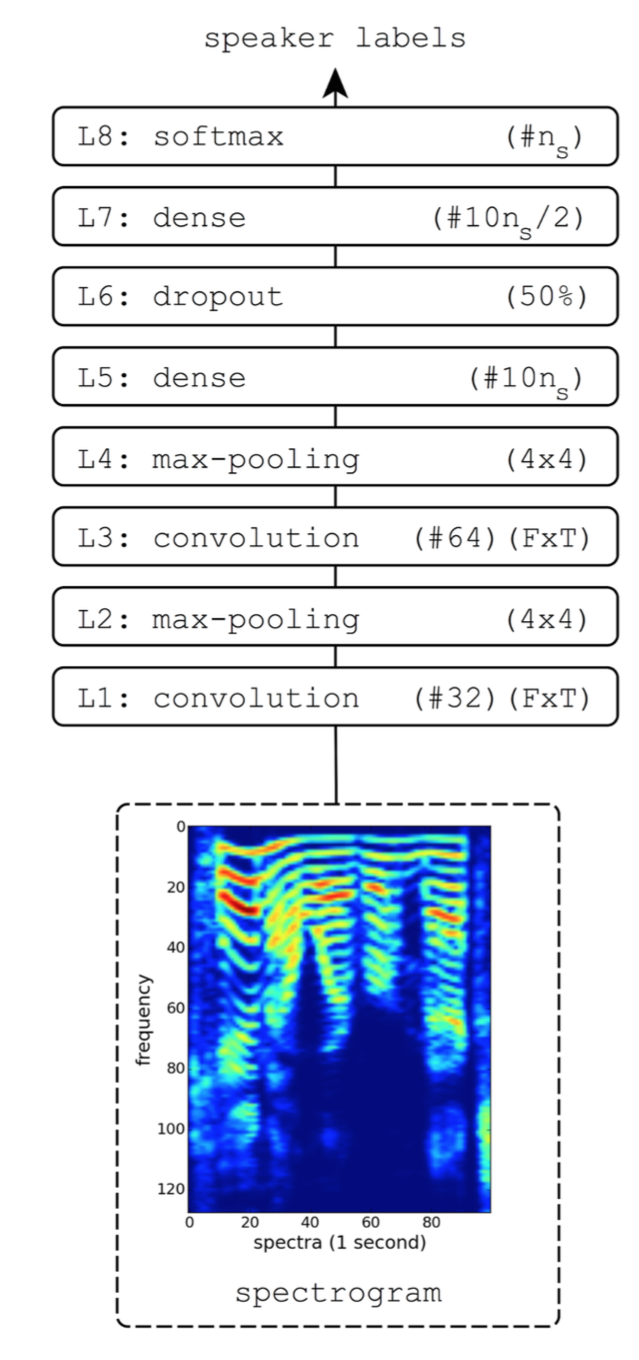
\includegraphics[width=0.25\textwidth]{./fig/cnn.png}
    \caption{Architecture for CNN speaker verifier}
    \label{fig:CNN}
\end{figure}

We train the CNN on our training set using 64*64 Mel-Spectrograms~\footnote{64 mel bands and 64 frames, 100 ms each} consisting of balanced samples from 101 speakers from the NIST 2004 and Blizzard datasets. Our model achieves 85\% test set accuracy.

\subsection{Adversarial attacks}
We define adversarial attacks on speaker recognition systems as \textit{targeted} or \textit{untargeted}. In
targeted attacks, an adversary is interested in designing an adversarial input
that makes the classification system predict a target class chosen by the
adversary. In untargeted attacks, the adversary is interested in a confident
prediction, regardless of the class being predicted. Untargeted attacks are essentially designed to fool the classifier into thinking a fake speech sample is real. Notice that a successful targeted attack is by definition a successful untargeted attack as well.
%
\section{Adapting Wasserstein GAN for Attacks}\label{sec:wgan}
In this section, we describe our generative adversarial network (GAN), and its usage as a speech recognition attacker. 
\subsection{Model}
The GAN framework proposed by~\cite{goodfellow2014generative} involves training a 
\textit{generator} network, which is trained to learn a function from noise to samples
that approximate the real data distribution. Simultaneously, a
\textit{discriminator} network is trained to identify whether a sample came from
the real distribution or not - i.e., it is trained to try to output 1 if a sample is real, and 0 if a sample is fake. The generator and discriminator can be arbitrary networks.

The GAN framework has been shown to be able to produce very realistic samples with low training overhead. However, since the generator is trained to minimize the Kullback-Leibler (KL) divergence between its constructed distribution and the real one, it suffers from an exploding loss term when the real distribution's support is not contained in the constructed one. To counter this, the \textit{Wasserstein GAN} \cite{arjovsky2017wasserstein} (WGAN) framework instead uses the Wasserstein (Earth-Mover) distance between distributions instead, which in many cases does not suffer from the same explosion of loss and gradient. Based on this, the loss functions of the generator and \textit{critic} (which no longer emits a simple probability, but rather an approximation of the Wasserstein distance between the fake distribution and real) become:
\begin{align}
    L_G &= -\underset{\boldsymbol{\widetilde{x}} \sim \mathbb{P}_{g}}{\mathbb{E}}  \big[D(\boldsymbol{\widetilde{x}})\big] \\
    L_C &= \underset{\boldsymbol{\widetilde{x}} \sim \mathbb{P}_{g}}{\mathbb{E}}  \big[D(\boldsymbol{\widetilde{x}})\big] - \underset{\boldsymbol{x} \sim \mathbb{P}_{r}}{\mathbb{E}}  \big[D(\boldsymbol{x})\big]
\end{align}
where $P_r$ is the real distribution and $P_g$ the learnt distribution of the generator. \\
The original WGAN framework uses weight clipping to ensure that the critic satisfies a Lipschitz condition. As pointed by \cite{gulrajani2017improved}, however, this clipping can lead to problems with gradient stability. Instead, \cite{gulrajani2017improved} suggest adding a gradient penalty to the critic's loss function, which indirectly tries to constrain the original critic's gradient to have a norm close to 1. Equation (2) thus becomes (taken from \cite{gulrajani2017improved}):
\begin{align}
    L_C &= \underbrace{\underset{\boldsymbol{\widetilde{x}} \sim \mathbb{P}_{g}}{\mathbb{E}}  \big[D(\boldsymbol{\widetilde{x}})\big] - \underset{\boldsymbol{x} \sim \mathbb{P}_{r}}{\mathbb{E}}  \big[D(\boldsymbol{x})\big]}_\text{Original critic loss}  + \underbrace{\lambda \underset{\boldsymbol{\hat{x}} \sim \mathbb{P}_{\hat{x}}}{\mathbb{E}}  \big[(\lVert \nabla_{\boldsymbol{\hat{x}}} D(\boldsymbol{\hat{x}}) \rVert_2 - 1)^2\big]}_\text{Gradient Penalty}
\end{align} \\
In all of our experiments, we use the Wasserstein GAN with this gradient penalty (WGAN-GP), which we found makes the model converge better than regular WGAN or GAN. We will henceforth use WGAN, GAN, and WGAN-GP interchangeably to refer to WGAN-GP.
\subsection{Attacks}
Performing \textit{untargeted} attacks with the WGAN-GP (i.e., training the network to output speech samples that mimic the distribution of speech) is relatively straightforward - we simply train the WGAN-GP using all speakers in our dataset. However, the most natural attack is one that is \textit{targeted}: where the GAN is trained to directly fool
a speaker recognition system, i.e., to produce samples that the system
classifies as matching a target speaker with reasonable confidence. \\
The first attempt was one in which we trained the WGAN-GP using data from only the target speaker. However, the generated samples did not fool
the speaker recognition systems, which was likely due to the discriminator's lack of access to data from other speakers. To circumvent this, we propose a 
modification to the critic's objective function that allows it to learn to 
differentiate between not only real samples and generated samples, but also between real speech samples from a target 
speaker and real speech samples from other speakers. We do this by adding a term 
to the critic's loss that encourages its discriminator to classify real speech 
samples from untargeted speakers as fake. From (3), the critic's loss $L_C$ changes to:
\begin{align}
    \underbrace{\underset{\boldsymbol{\widetilde{x}} \sim \mathbb{P}_{g}}{\mathbb{E}}  \big[D(\boldsymbol{\widetilde{x}})\big]}_\text{Generated Samples} \color{red} + \alpha * \underbrace{\underset{\boldsymbol{\dot{x}} \sim \mathbb{P}_{\dot{x}}}{\mathbb{E}}  \big[D(\boldsymbol{\dot{x}})\big]}_\text{Different Speakers} \color{black} - \underbrace{\underset{\boldsymbol{x} \sim \mathbb{P}_{r}}{\mathbb{E}}  \big[D(\boldsymbol{x})\big]}_\text{Real Speaker}  + \underbrace{\lambda \underset{\boldsymbol{\hat{x}} \sim \mathbb{P}_{\hat{x}}}{\mathbb{E}}  \big[(\lVert \nabla_{\boldsymbol{\hat{x}}} D(\boldsymbol{\hat{x}}) \rVert_2 - 1)^2\big]}_\text{Gradient Penalty}
\end{align}
where $P_{\hat{x}}$ is the distribution of samples from other speakers and
$\alpha$ is a tunable scaling factor. 
%
\section{Experimental setup}\label{sec:experiments}\subsection{WGAN setup}
In our experiments, we trained a WGAN-GP
to produce spectrograms from 1 target speaker, against a set of over 100 "other" speakers. On each critic
iteration, we fed it with a batch of samples from one target speaker, 
and a batch of data uniformly sampled from the other speakers. \\ We used two popular
architectures for generator/critic pairs: 
\begin{itemize}
    \item \textit{DCGAN}~\cite{radford2015unsupervised} models the generator as a series of deconvolutional layers with ReLU activations, and the discriminator as a series of convolutional ones with leaky ReLU activations. Both architectures use batch normalization after each layer.
    \item \textit{ResNet}~\cite{ledig2016photo} models the generator and discriminator each as very deep convnets (30 layers in our experiments) with upsampling/downsampling respectively. Residual (skip) connections are added every few layers to make training easier.
\end{itemize}
Initially, we were able to converge the targeted loss model used the same parameters as \cite{gulrajani2017improved}, namely 5 critic iterations per generator iteration, a gradient penalty weight of 10, and batch size of 64. Both the generator and critic were trained using the Adam optimizer \cite{kingma2014adam}. However, under these parameters we found that the highest $\alpha$ weight we could successfully use was 0.1 (we found that not including this scaling factor led to serious overfitting and poor convergence of the GAN). \\ The drawback of this approach is that the critic is not fully trained to discriminate against other speakers' data. In order to converge a model with $\alpha$ as 1, we made several modifications to 
the network parameters. We changed the standard deviation of the DCGAN discriminator's weights to be 0.05. To accommodate the critic's access to additional data in the mixed loss function (4), we increased the generator's learning rate to $1e^{-4}$, whereas the critic's learning rate was kept at $1e^{-5}$. Finally, we added of Gaussian noise to the target speaker data to prevent overfitting. 


\subsection{WaveNet}
Due to constraints on computing power, we used samples from WaveNet models that had been pre-trained for 88 thousand iterations. Parameters of the models were kept the same as those in \cite{van2016wavenet}. \\
The ability of WaveNet to perform \textit{untargeted} attacks amounts to using a model trained on an entire corpus. Targeted attacks are more difficult - we found that a single speaker's data was not enough to train WaveNet to converge successfully. To construct speaker-dependent samples, we relied on samples from pre-trained models that were \textit{globally conditioned} on speaker ID. Auditorily, such samples do sound very similar to the real speech of the ID in question. We ran the feature-extraction in section 3 on these samples to produce data fed to the classifier.
 
% subsection WaveNet (end)
\subsection{sampleRNN} % (fold)
Similarly to WaveNet, we found that the best (least noisy) sampleRNN samples came from models which were pretrained with a high number of iterations. Accordingly, we obtained samples from the three-tiered architecture, trained on the
Blizzard 2013 dataset \cite{prahallad2013blizzard}, which as mentioned in Section 3 is a 300 hour corpus of a single female speaker's narration. We also downloaded 10 second samples from the original paper's online repository at
\texttt{https://soundcloud.com/samplernn/sets}, which we qualitatively found to have less noise than our generated ones. 
% subsection SampleRNN (end)

%
\section{Results}
\label{sec:results}
\subsection{GAN Mel-Spectrogram}
Using the improved Wasserstein GANs framework, we trained generators to
construct 64x64 mel-spectrogram images from a noise vector. Visual results are demonstrated below in Figure~\ref{fig:samples_comparison}.   We saw recognizable Mel-Spectrogram-like features in the
data after only 1000 generator iterations, and after 5000 iterations the generated samples were indistinguishable from real ones. Training took around 10
hours for 20000 iterations on a single 4 GB Nvidia GK104GL GPU.
\begin{figure}[h]
    \centering
    \begin{subfigure}[b]{0.4\textwidth}
        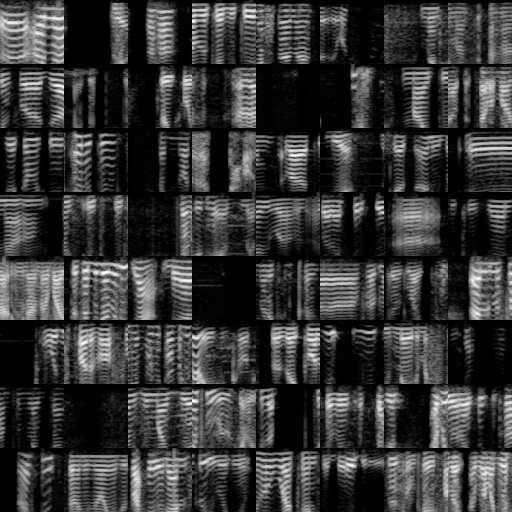
\includegraphics[width=\textwidth]{./fig/samples_groundtruth.png}
        \caption{Real (actual)}
        \label{fig:samples_real}
    \end{subfigure}
    \qquad
    \begin{subfigure}[b]{0.4\textwidth}
        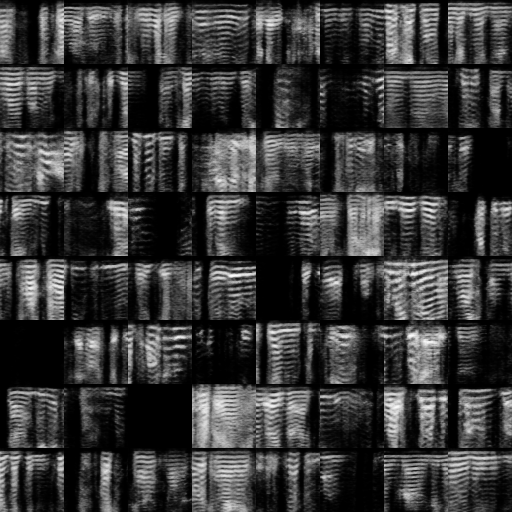
\includegraphics[width=\textwidth]{./fig/samples_5419.png}
        \caption{Fake (generated)}
        \label{fig:samples_fake}
    \end{subfigure}
    \caption{Comparison of real and generated ($\sim$ 5000 generator iterations)
    spectrogram samples from all speakers. Each grid contains 64 samples.}
    \label{fig:samples_comparison}
\end{figure}

\subsection{GAN Adversarial attacks}

Within the GAN framework, we train models for untargeted attacks by using all
data available from speakers that the speaker recognition systems was trained on, 
irrespective of class label. We show that an untargeted model able to generate 
data from the real distribution with enough variety can be used to perform 
adversarial attacks. We provide details in the untargeted attacks 
subsection \ref{sub:untargeted}. Figure~\ref{fig:histogram_untargeted} depicts
that our GAN-trained generator successfully learns all speakers across the
dataset, without mode collapsing.
\begin{figure}[t]
    \centering
    \begin{subfigure}[b]{0.4\textwidth}
        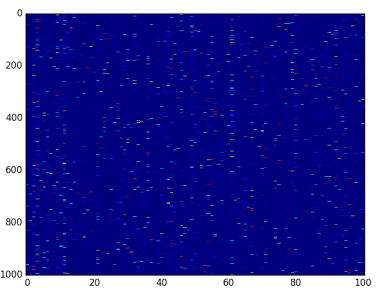
\includegraphics[width=\textwidth]{./fig/conf_mat_untargeted.png}
        \caption{Our speaker classifier's softmax distribution of 1000 samples 
        on approximately 100 speakers.}
        \label{fig:cm_untargeted}
    \end{subfigure}
    \qquad
    \begin{subfigure}[b]{0.4\textwidth}
        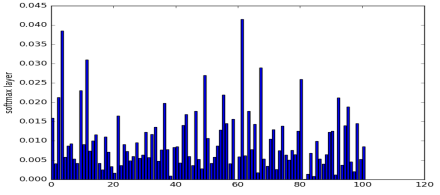
\includegraphics[width=\textwidth]{./fig/histogram_untargeted.png}
        \caption{Our speaker classifier's distribution of randomly sampled 
        speech from the generative model.}
        \label{fig:histogram_untargeted}
    \end{subfigure}
    \qquad
    \begin{subfigure}[b]{0.3\textwidth}
        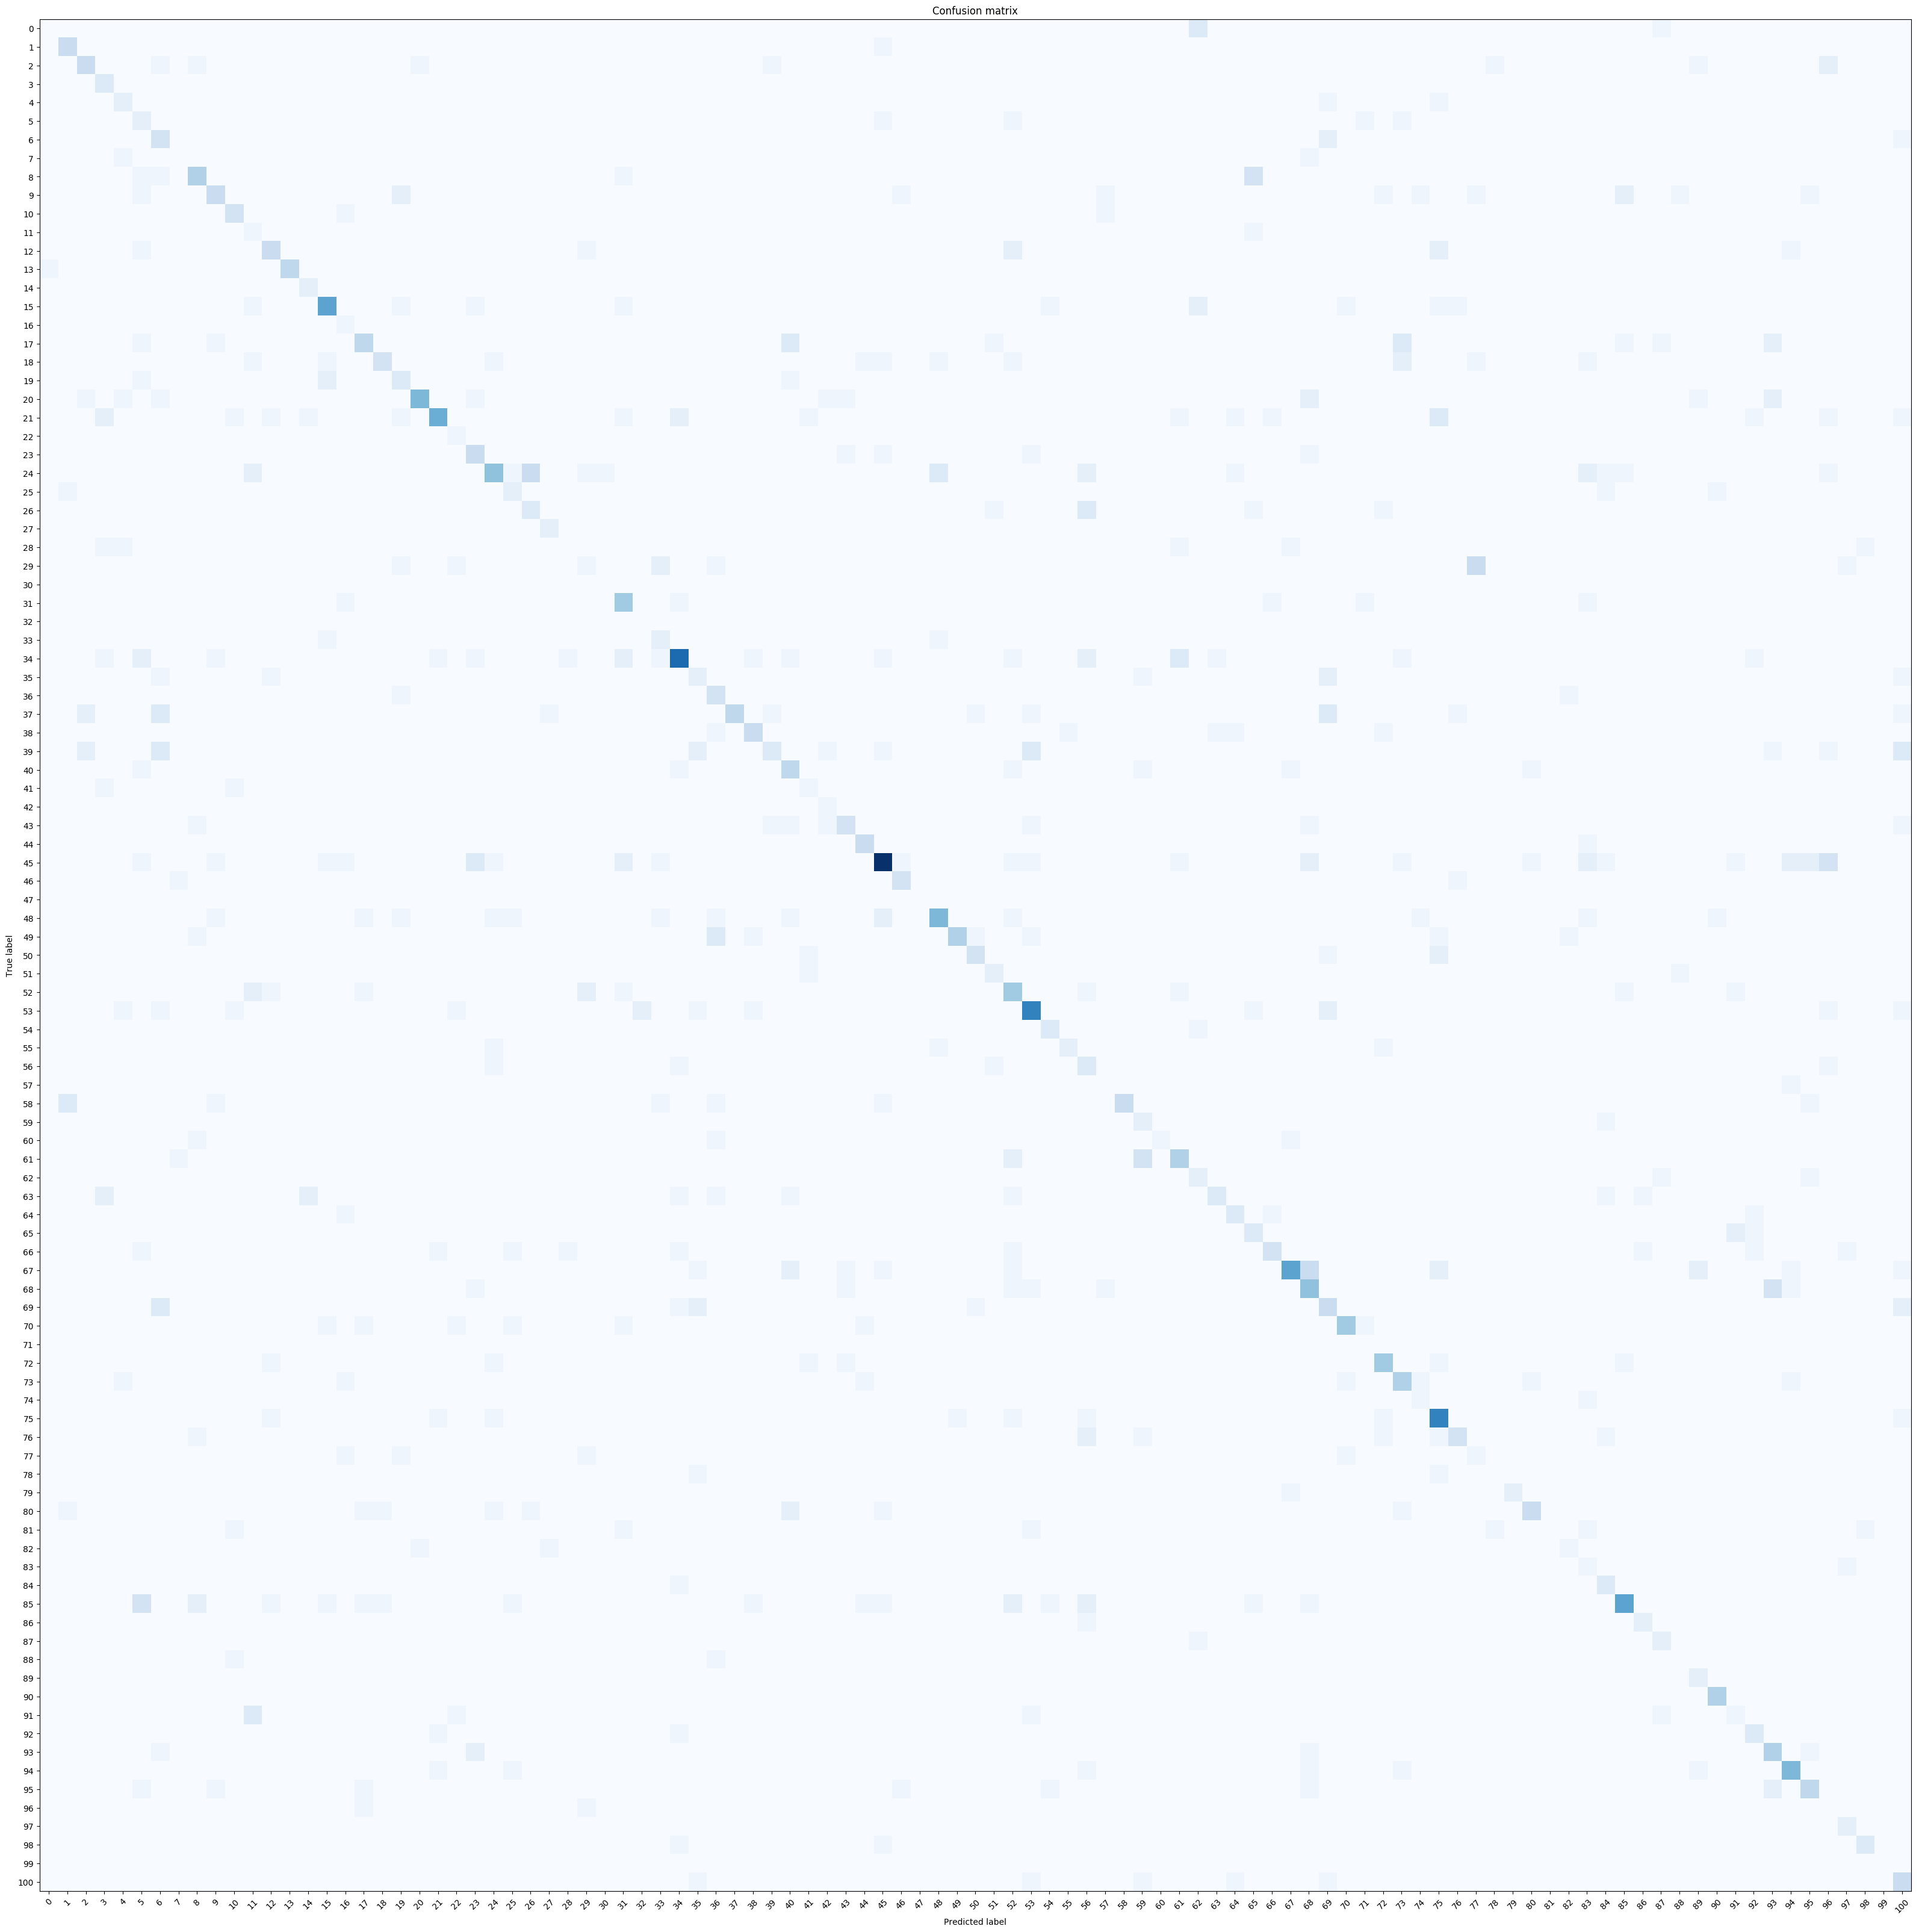
\includegraphics[width=\textwidth]{./fig/conf_mat_cnn_knn.png}
        \caption{Confusion matrix of untargeted model. x-axis corresponds to predicted label, y-axis to ground truth.}
        \label{fig:histogram_untargeted}
    \end{subfigure}
    \caption{Summary of untargeted attacks. Red represents high confidence.}
    \label{fig:conf_mat_cnn_knn}
\end{figure}

As we described earlier, the models for targeted attacks can be trained in two manners: 1) 
conditioning the model on additional information, e.g. class labels, as
described in~\cite{mirza2014conditional}; 2) using only data from the label 
of interest. While the first approach might result in mode collapse, a drawback
of the second approach is that the discriminator, and by consequence the
generator, does not have access to universal\footnote{We draw a parallel with 
Universal Background Models in speech.} properties of speech. In the targeted 
attacks subsection \ref{sub:targeted} we show results using our a new objective function that allows 
using data from all speakers.  

\subsubsection{Untargeted attacks}
\label{sub:untargeted}
For each speaker audio data in the test set, we compute a Mel-Spectrogram as
descibred in section \ref{sub:processdata}. The resulting Mel-Spectrogram is
then fed into the CNN recognizer and we extract a 505-dimensional feature $G$ from
the penultimate fully-connected layer (L7) in the pre-trained CNN model
(\ref{fig:CNN}) trained on the train partition of the real speech dataset with all 
speaker IDs.  This deep feature/embedding $G$ is then used to train a 
K-nearest-neighbor (KNN) classifier, with K equal to 5.

To control the generator trained by our WGAN, we feed the generated
Mel-Spectrograms into the same CNN-L2 pipeline to extract their corresponding
feature $\widehat G$. Utilizing the pre-trained KNN, each sample is assigned to
the nearest speaker in the deep feature space. Therefore, we know which speaker
our generated sample belongs to when we attack our CNN recognizer. We evaluate our
controlled WGAN samples against the state-of-the-art CNN recognizer, and the
confusion matrix can be found in Figure \ref{fig:conf_mat_cnn_knn}. 


\subsubsection{Targeted attacks}
\label{sub:targeted}
We ran all three models (WGAN-GP, SampleRNN, WaveNet) on a mixed corpus containing the entirety of the NIST 2004 corpus, a single speaker (280) from the VCTK Corpus, and the single speaker from the Blizzard dataset. The mixed corpus therefore contains 102 speakers. Samples were created from WaveNet globally conditioned on the single VCTK corpus speaker, and on SampleRNN trained only on data from the Blizzard dataset.
Results are demonstrated in Figure
\ref{fig:confusion_matrices}. Neither WaveNet samples nor sampleRNN samples
were able to attack the recognition model in the same way. In both models, \textbf{none} of the predictions made by the classifier match the target speaker. \\ We also trained the WGAN-GP with mixed loss/without mixed loss on speaker 0. The histogram of predictions in Figure
~\ref{fig:pred_comp_spk0} shows that using the mixed loss model, most of the energy is concentrated on the target speaker 0. The improved WGAN-GP loss achieves 0.38 error
rate and our mixed loss achieves 0.12 error rate, producing a 75\%
increase in accuracy. It is therefore clear that the WGAN-GP mixed loss framework is an improvement on the original loss function, which is expected given the network's access to additional speaker data.

\begin{figure}[t]
    \centering
    \begin{subfigure}[b]{0.3\textwidth}
        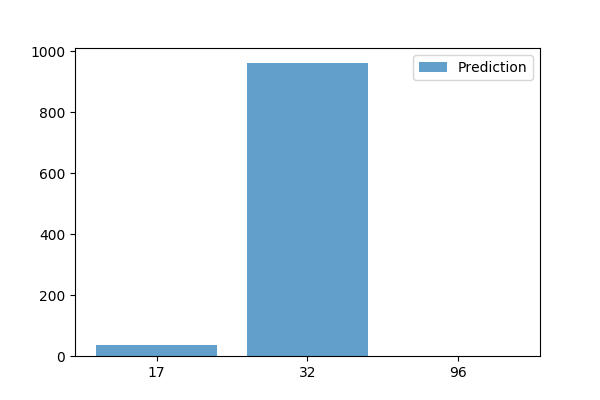
\includegraphics[width=\textwidth]{./fig/pred_histogram_cathy.png}
        \caption{Histogram of sampleRNN predictions. \textbf{Ground truth label: 100}.}
        \label{fig:pred_sampleRNN}
    \end{subfigure}
    \quad
    \begin{subfigure}[b]{0.3\textwidth}
        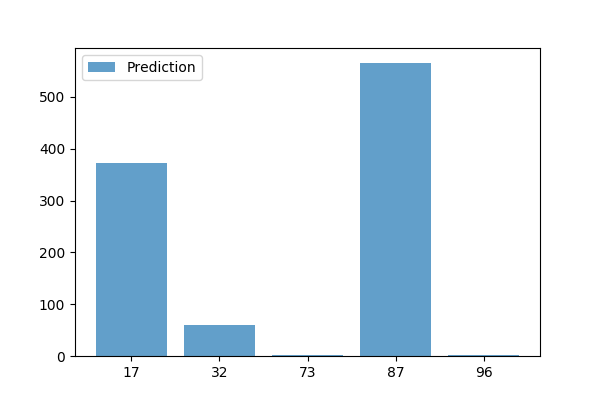
\includegraphics[width=\textwidth]{./fig/pred_histogram_p280.png}
        \caption{Histogram of WaveNet predictions. \textbf{Ground truth label: 101}.}
        \label{fig:pred_wavenet}
    \end{subfigure}
    \quad
    \begin{subfigure}[b]{0.4\textwidth}
        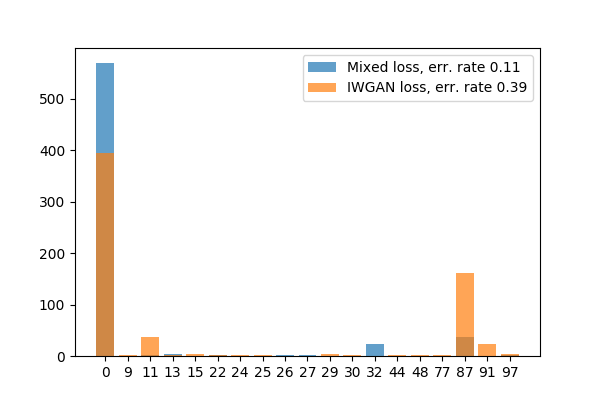
\includegraphics[width=\textwidth]{./fig/pred_comparisson_spk0.png}
        \caption{Histogram of predictions given improved WGAN and mixed loss models.}
        \label{fig:pred_comp_spk0}
    \end{subfigure}
    \caption{Summary histograms of targeted attacks}
    \label{fig:confusion_matrices}
\end{figure}

%
\section{Discussion and Conclusion}\label{sec:conclusions}
In this paper we have investigated the use of speech generative models to perform adversarial attacks on speaker recognition systems. We show that the autoregressive models we trained, i.e. SampleRNN and WaveNet, were not able to fool the CNN speaker recognizers we built. On the other hand, we show that adversarial examples generated with GAN networks are successful in performing targeted and untargeted adversarial attacks. 
%A pertinent argument against the validity of the GMM-UBM tests lies on the fact
%that GMM-UBM models have high precision and would not generalize to speech in
%different conditions, e.g. different room and microphone conditions. First, it
%is not within the scope of this paper to build a speaker recognition system
%that is invariant to room and microphone conditions. Second, given that the
%speaker recognition models, GMM-UBM and CNN, have good performance on test data
%and that WaveNet and SampleRNN goal is to replicate speech data that is from a
%speaker with similar and fixed microphone and room conditions, it is expected
%that the outputs of these generative models should be properly classified by
%the speaker recognition system.%

With this paper we hope to raise attention to issues that generative models bring to security and biometric systems. We foresee that samples produced with generative models have a signature that can be used to identify the source of the data and leave this investigation for future work.

%

\bibliographystyle{plain}
\bibliography{references.bib}

\end{document}
